\documentclass[12pt, a4paper, oneside]{vitmscthesis}

\thesistitle{An Approach for Extracting and Replicating Table Data from PDF Sources}
\thesison{Master Thesis}
\programme{M.Sc. Data Science}
\programmeLongName{Master of Science in Data Science}
\department{Department of Mathematics}
\school{School of Advanced Sciences}
\student{Ankita Sarkar}
\regno{22MDT1067}
\guide{Dr.\,David Raj Micheal}
\hod{Dr.\,K Muthunagai}
\submittedon{April - 2024}
\bibliographyname{References}

\begin{document}
	
%%%-----Printing the first few pages:  title, certificate, acknowledgment, etc.
\pagenumbering{roman}
%
%******************************************************
%
\begin{titlepage}
\centering

\emph{A project report on}

{ \LARGE \bfseries\MakeUppercase{\printtitle}}\\[1.5cm]


%\begin{large}\sffamily 
%\thethesison
%\end{large} \\[1cm]




{\large Submitted in partial fulfillment for the award of the degree of }\\ [1.5cm]

{\huge \bfseries \theprogrammeLongName}\\ [1.0cm]

{\large by} \\[1.5cm]

%
%   Name of author
% 
{\Large  \bfseries \MakeUppercase{\thestudent}}\\
{\large \bfseries  (Reg. No. \theregno)}\\ [1.5cm]

%\normalsize {in } \\ [0.5cm]

%{\large \sf  Software Engineering}\\ [1.0cm]
%

\vfill
%   Bottom of the page
%   
%   Logo
%
\includegraphics[width=0.4\textwidth]%
{img/vitcclogo}\\[0.3cm]
%
%   Department particulars
%
%{\large  \bfseries \thedepartment }\\
{\Large  \bfseries \MakeUppercase{\theschool} }\\
%{\large  Vellore Institute of Technology,  Chennai\\ 
%\normalsize Vandalur - Kelambakkam Road, Chennai - 600 127}\\[1ex] 
%({ \bf \tt http://www.vit.ac.in})\\[0.5cm]
\bigskip
{\thesubmittedon }

%

\end{titlepage}
%
%******************************************************
%


\thispagestyle{plain}

\vspace*{-3\baselineskip}
\begin{center}
	
\includegraphics[width=0.5\textwidth]{img/vitlogo}\\[0.3cm]
	
{\Large \bf DECLARATION}\\[0.75cm]
\addcontentsline{toc}{chapter}{Declaration}
\index{declaration}
\end{center}


%%   Declaration statement
%%
I hereby declare that the project entitled 
{\bf \printtitle} 
submitted by me to the Department of Mathematics, School of Advanced Sciences, Vellore Institute of Technology, Chennai, 600\;127 
in partial fulfillment of the requirements of the award of the degree of {\bf \theprogrammeLongName} 
is a bona-fide record of the work  
carried out by me under the supervision of {\bf \theguide}. 
I further declare that 
the work reported in this project, has not been submitted and will not be submitted,
either in part or in full, for the award of any other degree or diploma of this
institute or of any other institute or University.

%

%
%   Spaces for signature 
%

\vspace{3\baselineskip}

\begin{minipage}{.5\textwidth}
	\raggedright
	\begin{tabular}{lcl}
		\textbf{Place}  & : & Chennai \\
		\textbf{Date} & : &
	\end{tabular}
\end{minipage}%
\begin{minipage}{.5\textwidth}
	\raggedleft
	\thestudent\\
	Reg. No: \theregno\\
\end{minipage}

\cleardoublepage



\thispagestyle{plain}
\addcontentsline{toc}{chapter}{Certificate}

\vspace*{-3\baselineskip}
\begin{center}
	\includegraphics[width=0.4\textwidth]%
	{img/vitcclogo}\\[0.3cm]
	{\Large  \bfseries {\theschool} }\\[.3cm]
{\Large \bf CERTIFICATE}
\end{center}
\index{certificate}

%
%   Certificate statement
%
This is to certify that the thesis entitled {\bf \printtitle} is prepared and 
submitted by {\bf \thestudent\  
(Reg. No. \theregno)}
to Vellore Institute of Technology, Chennai, in partial fulfillment of the requirement for the award of
the degree of {\bf \theprogrammeLongName} 
is a bona-fide record carried out under my guidance.
The project fulfills the requirements as per the regulations of this
University and in my opinion meets the necessary standards for submission.
The contents of this report have not been submitted and will not be submitted
either in part or in full, for the award of any other degree or diploma
and the same is certified.
%
%   Spaces for signatures 
%

\begingroup
\linespread{1} \selectfont

\vspace{3\baselineskip}

\noindent\begin{minipage}{.5\textwidth}
	\raggedright
	\begin{tabular}{lcl}
			Signature of Guide&: & 	\\
			Name & : & 	{\bf \theguide}\\
		Date  & : &  \\
	\end{tabular}
\end{minipage}%

\vspace{4\baselineskip}

\noindent \begin{minipage}{.5\linewidth}
	\raggedright
	\begin{tabular}{lcl}
		\multicolumn{3}{c}{Signature of Internal Examiner}\\
		Name & : & 	\\
		Date  & : &  \\
	\end{tabular}
\end{minipage}%
\begin{minipage}{.5\linewidth}
	\raggedleft
	\begin{tabular}{lcl}
			\multicolumn{3}{c}{Signature of External Examiner}\\
		Name & : & 	\\
		Date  & : &  \\
	\end{tabular}
\end{minipage}%

\vspace{3\baselineskip}

\begin{minipage}[b]{.5\textwidth}
~
%(School Seal)
\end{minipage}%
\begin{minipage}[b]{.5\textwidth}
	\raggedleft
	
	Approved by the Head of Department\\
	{\bfseries\theprogramme} \\[2\baselineskip]
	
		\begin{tabular}{lcl}
		Name & : & \thehod	\\
		Date  & : &  \\
	\end{tabular}
\end{minipage}

\endgroup
\raggedbottom
\cleardoublepage
%
%   End of Certificate
%  


\thispagestyle{plain}
\addcontentsline{toc}{chapter}{Acknowledgement}
\begin{center}
	{\Large \bf \MakeUppercase{Acknowledgement}}
\end{center}
\index{acknowledgment}

With immense pleasure and a deep sense of gratitude, I wish to express my sincere thanks to my supervisor \emph{\theguide}, Assistant Professor, School of Advanced Sciences, Vellore Institute of Technology (VIT), Chennai for his motivation and continuous encouragement, this project would not have been successfully completed.

 I am grateful to the Chancellor of VIT, {\em Dr. G.Viswanathan}, the Vice Presidents {\em Mr. Sankar Viswanathan}, {\em Dr. Sekar Viswanathan}, {\em Dr. G V Selvam}, the Executive Director, {\em Dr. Sandhya Pentareddy} , the Assistant Vice President {\em Ms. Kadhambari S. Viswanathan} the Vice Chancellor {\em Dr. V. S. Kanchana Bhaaskaran}, the Pro Vice Chancellor of VIT Chennai {\em Dr. T. Thyagarajan} and the Additional Registrar {\em Dr. P. K. Manoharan} for motivating me to carry out the project at Vellore Institute of Technology, Chennai.

 I express my sincere thanks to {\em Dr. S. Mahalakshmi}, Dean, School of Advanced Sciences, VIT, Chennai and {\em Dr. K. Muthunagai}, HOD, Mathematics and Computing, School of Advanced Science,  VIT, Chennai for their support and encouragement.


 I wish to extend my profound sense of gratitude to {\em my parents} for providing me the moral support and encouragement whenever required.   



\vspace{3\baselineskip}

\begingroup
\linespread{1} \selectfont

\begin{minipage}{.5\textwidth}
	\raggedright
	\begin{tabular}{lcl}
		\textbf{Place}  & : & Chennai \\
		\textbf{Date} & : &
	\end{tabular}
\end{minipage}%
\begin{minipage}{.5\textwidth}
		\raggedleft
		\thestudent\\
		Reg. No: \theregno\\
\end{minipage}

 \endgroup


\chapter*{Abstract}
\addcontentsline{toc}{chapter}{Abstract}

Abstract to your work. \cite{bar}

\begin{keywords}
	Machine Learning, Deep Learning...
\end{keywords}



\tableofcontents

\listoftables 
\listoffigures

%%--- All chapters
\mainmatter
\chapter{Introduction}

The introduction is a shorter version of the rest of the report, and in many cases the rest of the report can 
also have the same flow that summarizes the major contributions of the project. The chapter should provide a 
critical and concise outline of the subject to be covered by the dissertation and indicate how this study will 
contribute to the subject. This chapter should include the descriptions such as: (not necessarily in that order, 
but what is given below is a logical order). Example of a citation: \cite{bar}
\begin{itemize}
	\item Background [The setting of the scene of the problem].
	\item Statement [Exact problem you are trying to solve]. 
	\item Motivation [Importance of the problem]. 
	\item Post/Related work [Existing methods including pros and cons of the methods should be cited wherever possible].
	\item Challenges [Difficulty in the problem solving].
	\item Essence of your approach [Your method of problem solving].
	\item Statement of assumptions [The conditions under which your solution is applicable].  
	\item Organization of the report. 
	\item Aim(s) and Objective(s)
	\item Avoid ‘routine’ background e.g. the C programming language.
	\item Don’t cite endless sources that are irrelevant or that you haven’t read.
\end{itemize}



\chapter{Literature Review }

Deep learning has revolutionized artificial intelligence, enabling significant breakthroughs in various domains. 

The foundation of modern deep learning is well captured by \citeauthor{goodfellow2016deep} in their book \cite{goodfellow2016deep}, where they provide an extensive discussion on neural networks, optimization strategies, and deep architectures. This work serves as a comprehensive resource on the mathematical and practical aspects of deep learning.


In \citeyear{he2016deep}, \citeauthor{he2016deep} introduced the concept of deep residual learning in \cite{he2016deep}. Their work addresses the challenges of training very deep neural networks by introducing residual connections, which help mitigate the vanishing gradient problem. By using identity mappings, the proposed residual networks (ResNets) allow for more effective gradient flow, leading to significant improvements in deep model training. Their architecture achieved state-of-the-art performance on benchmark datasets such as ImageNet, demonstrating the importance of deeper networks in advancing computer vision tasks.

\section{Mathematical Formulation}
The research problem can be expressed as:
\begin{equation}
	E = mc^2
\end{equation}
where $E$ is energy, $m$ is mass, and $c$ is the speed of light.


\section{Tables and Figures}
Table~\ref{tab:example} presents some sample data.

\begin{table}[h]
	\centering
	\begin{tabular}{l c c}
		\toprule
		Category & Value 1 & Value 2 \\
		\midrule
		A & 10 & 20 \\
		B & 15 & 25 \\
		C & 20 & 30 \\
		\bottomrule
	\end{tabular}
	\caption{An example table.}
	\label{tab:example}
\end{table}

Figure~\ref{fig:example} illustrates an example image.


\begin{table}[h]
	\centering
	\rowcolors[\hline]{2}{green!30}{yellow!50} %alternate row colors starting at row 2
	 \arrayrulecolor{red} % border color
	 \setlength\arrayrulewidth{1.2pt} %  border size
	\begin{tabular}{|l| c| c|}
		\hline
	\rowcolor{pink} 	Category & Value 1 & Value 2 \\
		\hline
		  A & 10 & 20 \\ \hline 
		 B & 15 & 25 \\ \hline 
		   C & 20 & 30 \\ 
		\hline
				   D & 10 & 50 \\ 
		\hline
				   E & 50 & 80 \\ 
		\hline
	\end{tabular}
	\caption{An example table with some colors.}
	\label{tab:example2}
\end{table}


\begin{figure}[h]
	\centering
	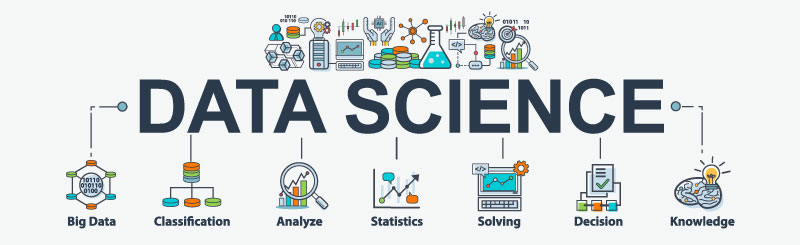
\includegraphics[width=0.75\textwidth]{img/data-science}
	\caption{An example figure.}
	\label{fig:example}
\end{figure}

\section{Enumerations}
Important points to consider:
\begin{enumerate}
	\item First point.
	\item Second point.
	\item Third point.
\end{enumerate}

Enumerations with alpha numerics.
\begin{enumerate}[label={(\alph*)}]
	\item First point.
	\item Second point.
	\item Third point.
\end{enumerate}


Roman Enumerates.

\begin{enumerate}[label={(\roman*)}]
	\item First point.
	\item Second point.
	\item Third point.
\end{enumerate}

\chapter{System Design}
The research problem can be expressed using fundamental equations in data science. One of the key formulations in machine learning is the cost function for linear regression:
\begin{equation}
	J(\theta) = \frac{1}{2m} \sum_{i=1}^{m} \left( h_\theta (x^{(i)}) - y^{(i)} \right)^2
\end{equation}
where:
\begin{itemize}
	\item $J(\theta)$ is the cost function,
	\item $h_\theta(x^{(i)})$ is the hypothesis function,
	\item $y^{(i)}$ is the actual value,
	\item $m$ is the number of training examples.
\end{itemize}

Another fundamental concept in deep learning is the softmax function used in classification:
\begin{equation}
	\sigma(z)_j = \frac{e^{z_j}}{\sum_{k=1}^{K} e^{z_k}}
\end{equation}
where $z$ is the input vector and $K$ is the number of classes.

Matrices play a crucial role in data science, especially in neural networks. A typical forward propagation step in a neural network can be expressed as:
\begin{equation}
	A^{[l]} = g(W^{[l]} A^{[l-1]} + b^{[l]})
\end{equation}
where:
\begin{description}
	\item $A^{[l]}$ is the activation at layer $l$,
	\item $W^{[l]}$ is the weight matrix,
	\item $b^{[l]}$ is the bias vector,
	\item $g(\cdot)$ is the activation function.
\end{description}

An example of a weight matrix in a neural network with three inputs and two neurons is:
\begin{equation}
	W = \begin{bmatrix} 0.2 & 0.4 & 0.6 \\ 0.8 & 1.0 & 1.2 \end{bmatrix}
\end{equation}

\section{Typing theorems and definitions}
\begin{definition}[Probability Distribution]
	A probability distribution is a function that provides the probabilities of occurrence of different possible outcomes in an experiment. Formally, for a discrete random variable $X$, the probability mass function (PMF) is defined as:
	\begin{equation}
		P(X = x) = f(x), \quad \sum_{x} f(x) = 1.
	\end{equation}
\end{definition}

\begin{lemma}[Universal Approximation Theorem]
	A feedforward neural network with a single hidden layer containing a finite number of neurons can approximate any continuous function on a compact subset of $\mathbb{R}^n$, provided the activation function is non-constant, bounded, and monotonically increasing.
\end{lemma}

\begin{theorem}[Central Limit Theorem]
	Let $X_1, X_2, ..., X_n$ be a sequence of independent and identically distributed random variables with mean $\mu$ and variance $\sigma^2$. Then, as $n$ approaches infinity, the standardized sum:
	\begin{equation}
		Z_n = \frac{\sum_{i=1}^{n} X_i - n\mu}{\sigma\sqrt{n}}
	\end{equation}
	converges in distribution to the standard normal distribution:
	\begin{equation}
		Z_n \sim \mathcal{N}(0,1).
	\end{equation}
\end{theorem}

If you want more such environments to be numbered and formatted consistently, add the following code in the preamble of your document and replace the commands, what you need and use it as environments.

\begin{verbatim}
\newtheorem{corollary}[theorem]{Corollary}
\end{verbatim}
Note that, this follows the numbering of theorem environment. 

\begin{remark}
This remark is typed using the similar theorem environment but without numbering. Note that, we have added the following in the preamble to achieve this:
\begin{verbatim}
\newtheorem{remark}{Remark}
\end{verbatim}
\end{remark}


\chapter{Methodology}
This chapter should reflect development of the project such as: implementation, experimentation, optimization, evaluation etc. and unit integration testing should be discussed in detail.  The unit test cases and system test cases should describe the input, expected output and output obtained. It can also include the details of the tools used for implementation, justification for the selected tool and the detailed description of implemented modules.  Screen shots, Pseudocode etc. 
In case of simulation, modeling, programming techniques, programming steps, flow-charts, simulation results, verification of the approach followed and the like depending on the nature of the project. 
\section{Some section}
some dummy data is written here... Please change it according to your need...

The materials required, techniques followed, sample preparations, research design and methods should be clearly mentioned. The experimental procedure should be clearly defined.
\chapter{Results and Discussions}
This is part of the set of technical sections, and is usually a separate section for experimental/design papers.  This chapter should include:

\begin{itemize}
	\item Performance metrics.
	\item Parameters under study 
	\item Comparison of cases/ studies with respect to existing and proposed work / algorithm/ design–comparison/ with the published data and deviations / improvements if any as expected in the aims and objectives
	\item Expected and obtained results- Analysis of the results- statistical analysis, plots, simulated results, synthesis of process, interpretation of the results 
	\item Detailed results for each logical component of the project with an accompanying discussion section [Can include screen shots, graphs etc.].
	\item The results can be tabulated, graphically presented and photographs to be displayed if any.
	\item Discuss the results which should include an interpretation of the results and their relationship to the aims and objectives.
\end{itemize}
\chapter{Summary and Future Work}
This chapter should summarize the key aspects of your project (failures as well as successes) and should state the conclusions you have been able to draw.  Outline what you would do if given more time (future work).  Try to pinpoint any insights your project uncovered that might not have been obvious at the outset.  Discuss the success of the approach you adopted and the academic objectives you achieved.  Avoid meaningless conclusions, [e.g. NOT `` I learnt a lot about C++ programming ''].  Be realistic about potential future work.  Avoid the dreaded: ``All the objectives have been met and the project has been a complete success''.  You have to crisply state the main take-away points from your work.  Describe how your project is performed against planned outputs and performance targets.  Identify the benefits from the project.  Be careful to distinguish what you have done from what was there already.  It is also a good idea to point out how much more is waiting to be done in relation to a specific problem, or give suggestions for improvement or extensions to what you have done.  
Future scope of the work for improvement may also be included



\appendix

\chapter{Appendix Chapter}

Here is the appendix chapter. Usually, the code  and the other related items are given here. 



\addcontentsline{toc}{chapter}{\thebibliographyname}
\bibliography{reference}

%
\clearpage 
\thispagestyle{empty}
\vspace*{\fill}
\begin{flushright}
	\linespread{1}\selectfont
	
\includegraphics[width=0.35\textwidth]{img/vitlogo.png}\\[0.5cm]
	{\large \bf \sf  School of Advanced Sciences \ }\\
	{\sf Vellore Institute of Technology, Chennai\\
		Vandalur -- Kelambakkam Road, Chennai - 600 127\\
		(\url{www.chennai.vit.ac.in})}
\end{flushright}
%

\end{document}